\chapter{Implementation}\label{ch:implementation}

Given the requirements and the design in the previous chapters, refer to \cref{ch:requirements} and \cref{ch:design}, the project is implemented following the V-model established in \cref{ch:methodology_approach}. This chapter describes the implementation of the system, from the architecture to the deployment of the system.

\section{General Architecture}

The architecture, as seen in \cref{fig:architecture}, is composed of two main parts, the server and the communities. The server is in charge displaying the information to the users and the managers and handling the connection between the different communities. The communities are in charge of the detection of the vehicles, the opening of the gates, and the administration of the community (data storage, backup, etc).

\begin{figure}
	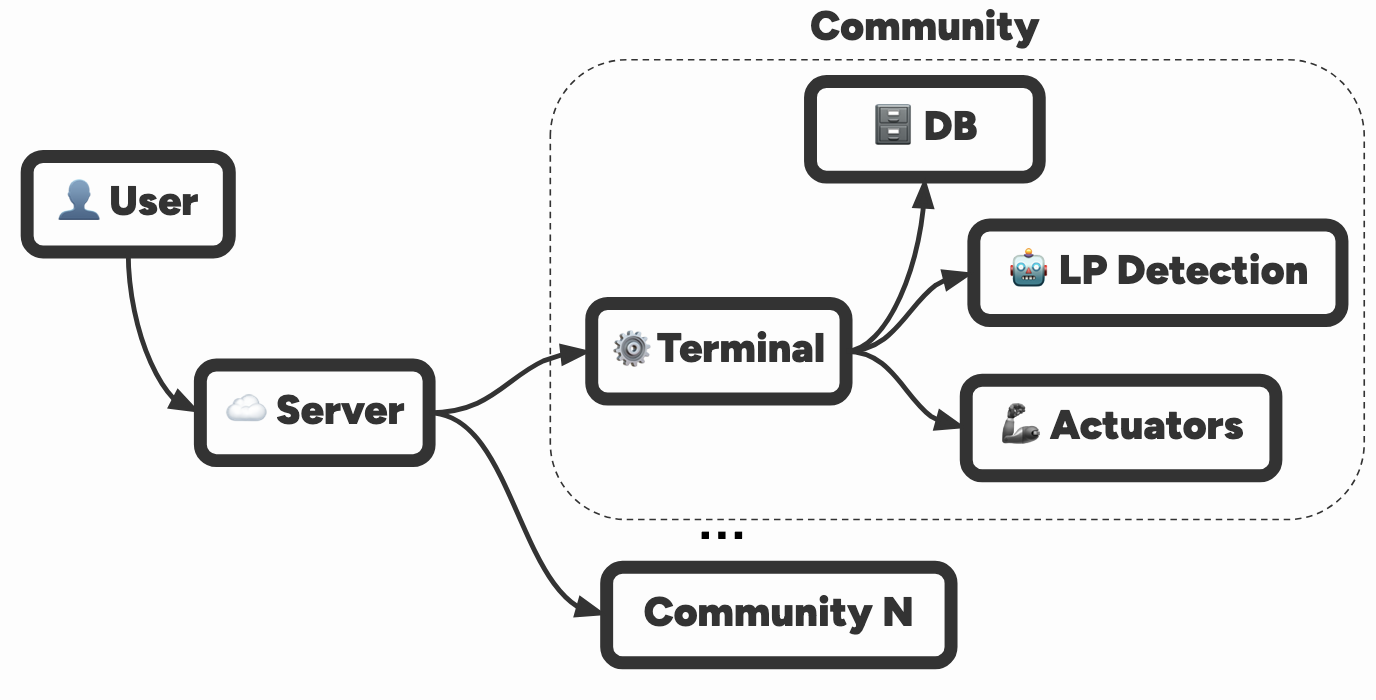
\includegraphics{architecture.png}
	\caption{General Architecture of the system}\label{fig:architecture}
\end{figure}

It is worth noting that the system is design to be scalable and robust, so the system is design to be able to be deployed in different communities and be able to handle the different data and users. That is why in \cref{fig:architecture} multiple communities can be seen.

\section{Community}

The community is a collection of the systems to provide the ability to open the gates, detect the vehicles, and store the data for a single building or community. A community is usually composed of three main subsystems, the licence plate detection system, the terminal server, and the actuators. Moreover, the community is connected to the internet to be able to connect to the server and perform other actions such as updates, remote administration, etc.

\subsection{Licence Plate Detection System}

The first component of the sytems is the detection of the licence plates. The detection of the licence plates is done by a deep learning algorithm that detects the licence plates in the images. The detection algorithm is based on YOLO \autocite{yolov8_ultralytics} and is implemented in the terminal. The detection algorithm is in charge of detecting the licence plates in the images and sending the data to the database.

The implementation of the algorithm is out of the scope of this project, and it is based on the Dual Licence Plate Recognition system \autocite{RAMAJOBALLESTER2024104608}. The system is composed of two main steps, the detection of the licence plate and the detection of the characters of the licence plate. Some examples can be seen in \cref{fig:licence_plate_detection}.

\begin{figure}
	\begin{subfigure}{0.95\textwidth}
		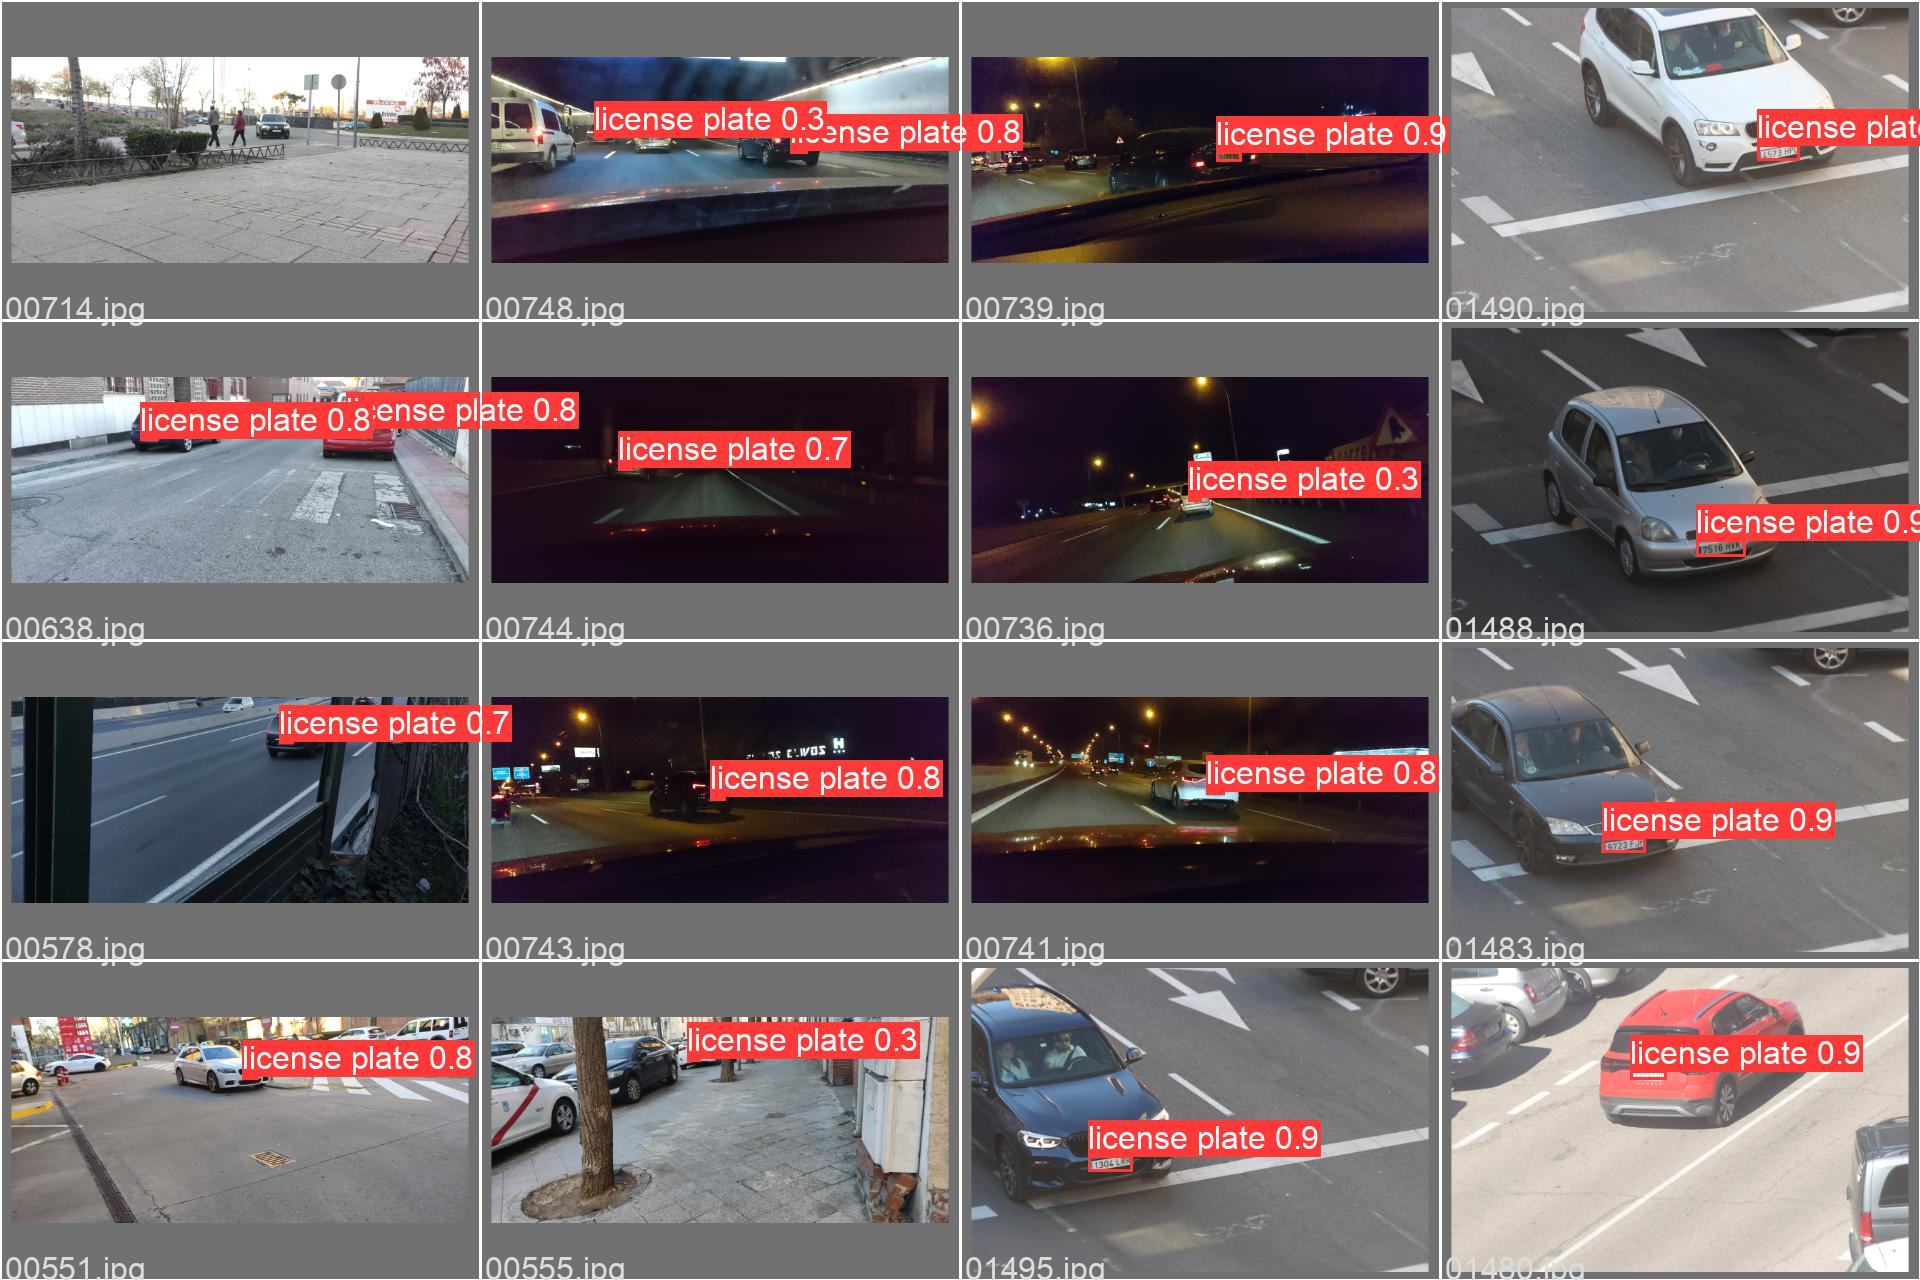
\includegraphics{licence_plate_recognition.jpg}
		\caption{Testing of the Licence Plate Detection System. \autocite{RAMAJOBALLESTER2024104608}}
	\end{subfigure}
	\br
	\begin{subfigure}{0.95\textwidth}
		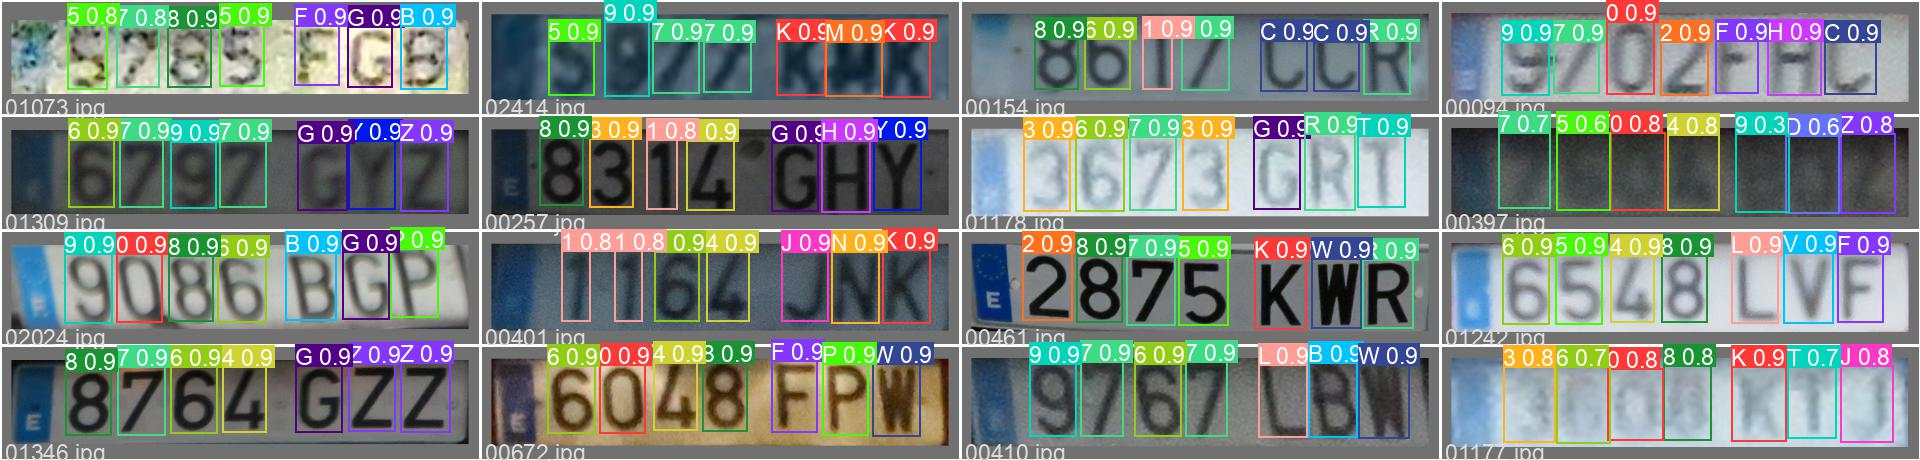
\includegraphics{ocr_licence_plate.jpg}
		\caption{Testing of the OCR character detection of the Licence Plate Detection System. \autocite{RAMAJOBALLESTER2024104608}}
	\end{subfigure}

	\caption{Licence Plate Detection alghorithms. \autocite{RAMAJOBALLESTER2024104608}}\label{fig:licence_plate_detection}
\end{figure}

\subsection{Terminal Server}

To provide the main functionality of the system, a terminal server is used. The terminal server is in charge of the communication between the different subsystems of the community and the server. The terminal server is in charge of communicating with the server, the actuators, the detection algorithm, the data storage, the backup of the data, and the user administration.

For reference, the terminal server is designed ot be run on any Linux system, and the implementation is based on the ExpressJS framework. This makes the terminal server easy to deploy and maintain. Moreover, the terminal server is design to be able to be updated remotely and be able to be connected to the internet.

For the communication between the different subsystems, the terminal server uses a RestAPI methodology. This allows the different subsystems to communicate with the terminal server and perform the different actions.

\subsubsection{Database}

Different architecture approaches were considered for the database, such as SQL or NoSQL databases, local or cloud databases. For this project, a local SQL database based on SQLite is used. The main reason behind this decision was the requirement of having the data inside the community for data privacy and security reasons. The SQL architecture is used as it provides a robust and reliable way to store the data and be able to perform the different actions required such as filtering, searching, and more. The database architecture can be seen in \cref{fig:database_architecture}.

\begin{figure}
	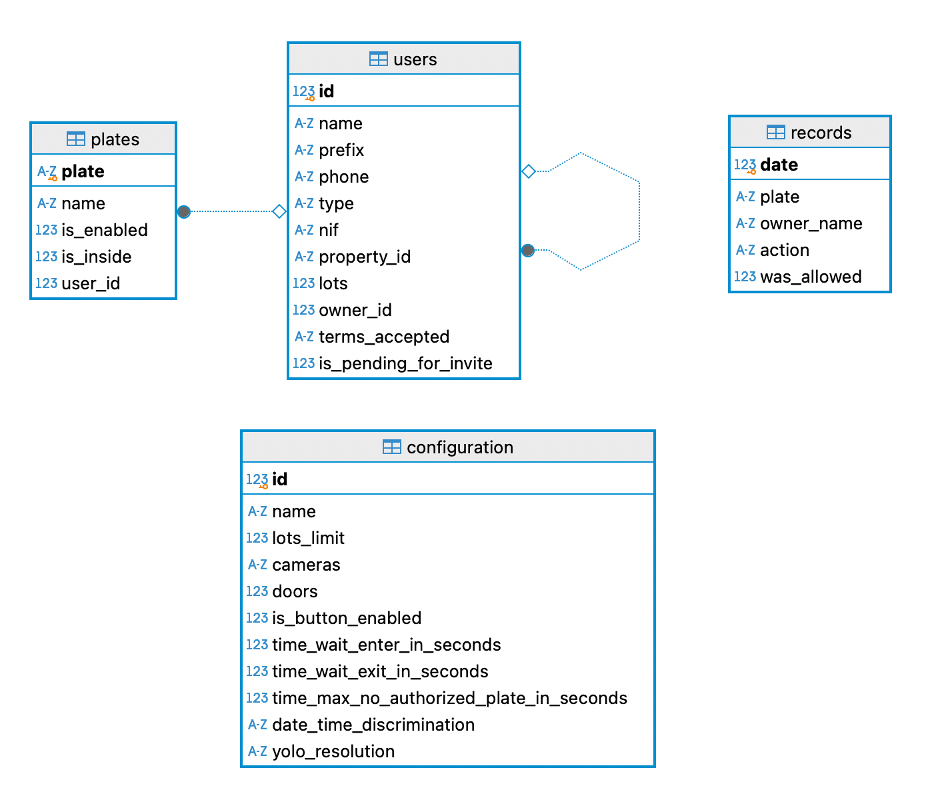
\includegraphics{database_architecture.png}
	\caption{Database Architecture}\label{fig:database_architecture}
\end{figure}

The database is divided into four main tables to store the different types of data.

The first table is the \texttt{users} table. This table is in charge of storing the information of the users of the system. The table is composed of the following fields:

\begin{itemize}
	\item \texttt{id}: The unique identifier of the user which is a autoincrement numeric field.
	\item \texttt{name}: The name of the user to identify it.
	\item \texttt{prefix}: The prefix of the phone used by the user, as the users come from different countries.
	\item \texttt{phone}: The phone number of the user.
	\item \texttt{type}: The type of the user, which can be either an administator, an owner of a property, or a visitor.
	\item \texttt{nif}: The NIF of the user, which is used to identify the user for regulatory and security reasons.
	\item \texttt{property\_id}: The identifier of the property of the user.
	\item \texttt{lots}: The number of parking spaces that the user has.
	\item \texttt{owner\_id}: Id of the owner of the property if the user is a visitor.
	\item \texttt{terms\_accepted}: A boolean field to check if the user has accepted the terms and conditions of the system.
	\item \texttt{is\_pending\_for\_invite}: A boolean field to check if the user is pending for an invitation to the system.
\end{itemize}

The primary key of the table is the \texttt{id} field. And a foreign key is used to connect the \texttt{owner\_id} field to the \texttt{id} field between an owner and a visitor. Moreover, different check are performed to ensure the data integrity and the security of the data, for example, the \texttt{phone} field is checked to be a valid phone number and unique.

Secondly, the \texttt{plates} table is used to store the information of the licence plates registed in the system. The table is composed of the following fields:

\begin{itemize}
	\item \texttt{plate}: Alphanumeric field to store the licence plate, the length is variable to adapt to different countries.
	\item \texttt{name}: Identifier of the licence plate for easy identification.
	\item \texttt{is\_enabled}: Boolean field to check if the licence plate is enabled or disabled, that is, if it is allowed to enter the community.
	\item \texttt{is\_inside}: Boolean field to check if the licence plate is inside the community in order to have a control of the vehicles inside the community.
	\item \texttt{user\_id}: The identifier of the user that owns the licence plate.
\end{itemize}

The primery key of the table is the \texttt{plate} field. A foreign key is used to connect the \texttt{user\_id} field to the \texttt{id} field of the \texttt{users} table. Moreover, the \texttt{plate} field is checked to be unique and the \texttt{user\_id} field is checked to be a valid user.

For the configuration of the community, the \texttt{configuration} table is used. The table is composed of the following fields:

\begin{itemize}
	\item \texttt{id}: The unique identifier of the configuration. As there is only one configuration, the field is a constant and set to 1 by default.
	\item \texttt{name}: The identifier name of the community.
	\item \texttt{lots\_limit}: The maximum number of parking spaces in the community.
	\item \texttt{cameras}: The configuration of the cameras in the community. It is used to match the specific cameras with the specific actuators of the community.
	\item \texttt{doors}: The number of garage doors in the community as multiple doors can be used for different points of the community.
	\item \texttt{is\_button\_enabled}: Boolean field to check if the button to open the door is enabled to be able to open the door manually.
	\item \texttt{time\_wait\_enter\_in\_seconds}: Timeout to wait for a vehicle to enter the community.
	\item \texttt{time\_wait\_exit\_in\_seconds}: Timeout to wait for a vehicle to exit the community.
	\item \texttt{time\_max\_no\_authorized\_plate\_in\_seconds}: Timeout to wait for a vehicle to enter the community if the licence plate is not authorized.
	\item \texttt{date\_time\_discrimination}: Variable to check if the system is using the date and time to discriminate the vehicles.
	\item \texttt{yolo\_resolution}: Configuration for the Licence Plate Detection System.
\end{itemize}

The primary key is the \texttt{id} field and it is set to 1 in order to only have one configuration. This information is kept in the database to centralized everything and make it easier to backup the data. A separate file can be used for the configuration, but it is stored in the database for security reasons.

Finally, the \texttt{records} table is used to store the logs of the system, that is all the different interactions with the different subsystems, such as the licence plates detected, the users that enter the community, the users that exit the community, etc. The table is composed of the following fields:

\begin{itemize}
	\item \texttt{date}: The timestamp of the record.
	\item \texttt{plate}: The licence plate of the vehicle that is detected.
	\item \texttt{owner\_name}: The name of the owner of the vehicle that is detected to have a better control of access flow.
	\item \texttt{action}: The action performed, that is, if the vehicle is entering or exiting the community.
	\item \texttt{was\_allowed}: Boolean field to check if the vehicle was allowed to enter the community.
\end{itemize}

The primary key of the table is the \texttt{date} field, this is done to restrict multiple different records for a sigle timestamp. Moreover, the \texttt{date} field is set to use the ISO 8601 format to have a standard format for the date and time.

As the terminal is situated in the community, unauthorized access to the database is a concern. To keep the database secured from unauthorized access, the database is encrypted using the SQLCipher library. This library is used to encrypt the database and ensure that the data is secure and only accessible by the system. Keeping the database encrypted ensures that the data is secure and only accessible by the system.

\subsubsection{Application Programming Interface}

As stated previously, in order to communicate with the different subsystems, a RestAPI is used. The RestAPI is used to perform the different actions such as opening the door, detecting the licence plates, storing the data, etc. The RestAPI is built using the ExpressJS framework, as it is easy to use and maintain. For this different endpoints are used to perform the different actions such as user administration, licence plate detection, door opening, etc. In order to perform the authenicaton of the users, JWT tokens are used to ensure that the request is performed by the right user. The authenicaton process is later outlined in \cref{sec:authentication}.

\subsubsection{Actuators}

To interact with the various subsystems of the communities, particularly for controlling access points like garage doors, the system employs a custom Relay Expansion Board designed for the NVIDIA Jetson Nano. This board serves as the interface between the digital control signals from the terminal server and the physical actuators. The choice of this solution came after studying different door opening systems, all of which required a signal to be pulled down to ground to trigger the mechanism.

The control of doors is achieved through relays, which act as electrically operated switches. To enable both automated and on-demand operation of the doors, a small server is set up within the terminal. This server listens for requests to open the door, which can come from either the license plate recognition system or authorized user commands.

When a valid request is received by the server, it processes the command and sends an appropriate signal to the Relay Expansion Board. The board then activates the corresponding relay, which in turn triggers the door mechanism to open. This setup allows for seamless integration of the automated license plate recognition system with manual override capabilities, ensuring flexibility and reliability in access control.

The use of relays provides several advantages. It offers electrical isolation between the control circuitry and the door mechanisms, allows for the control of high-voltage or high-current devices with low-voltage signals, and provides flexibility to adapt to various types of door actuators used in different communities.

This actuator subsystem is crucial in translating the software-based decisions of the parking management system into physical actions, effectively bridging the digital and physical aspects of the solution. The system's ability to open doors based on both automated detection and manual requests ensures a versatile and user-friendly operation, catering to different scenarios and user needs within the parking management ecosystem.

\subsubsection{Other subsystems}

The system incorporates several additional components that work together to ensure reliable operation and data integrity. The surveillance infrastructure utilizes a network of cameras strategically positioned throughout the community, particularly at entry and exit points. Each camera captures video feeds and transmits them to the terminal for processing using the Real-Time Streaming Protocol (RTSP). The cameras connect to the network infrastructure via Ethernet cables, ensuring stable and high-quality video transmission.

Network connectivity is managed through a dedicated 4G router equipped with an integrated switch. This router, specifically the TP-Link AC1200 model, serves two critical functions: it facilitates communication between the cameras and the terminal, and provides internet connectivity for the entire system. The choice of a 4G router ensures that the system remains independent of the community's existing infrastructure while maintaining reliable connectivity. The integrated switch allows for efficient connection of multiple cameras and the terminal, simplifying the network topology and reducing potential points of failure.

To ensure data integrity and business continuity, the system implements a comprehensive backup strategy. The database, which contains critical operational data including user information and access logs, is automatically backed up daily to Amazon S3 \autocite{AmazonS3}. These backups are encrypted both during transmission and storage, protecting sensitive information from unauthorized access. This automated backup system ensures a \gls{rpo} of 24 hours, minimizing potential data loss in the event of system failure or data corruption. The combination of local encrypted storage and cloud-based backups provides a robust solution for data protection and recovery.

\section{Cloud deployment}

To enable the access to the different communities from the user point of view, a web server is deployed in AWS. The main component is a NextJS server that holds the website that the users use to access the system and also the backend functionality to connect to each specific community.

\subsection{Cloud Architecture}

The cloud architecture developed for this project adopts a cost-effective and scalable methodology, leveraging Amazon Web Services (AWS) as the primary cloud provider. As illustrated in \cref{fig:cloud_architecture}, the architecture employs a distributed design that prioritizes reliability and security while maintaining operational efficiency.

\begin{figure}
	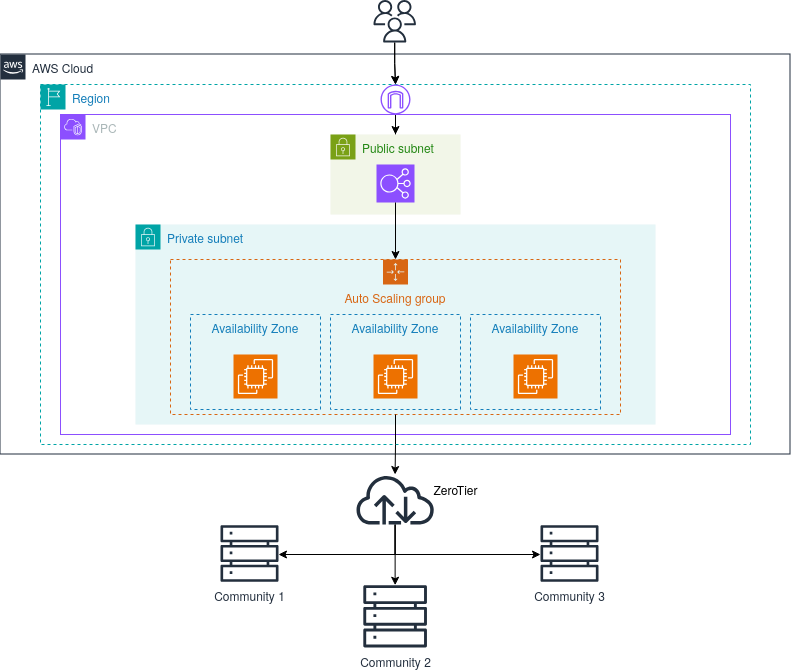
\includegraphics{cloud_architecture.png}
	\caption{AWS Cloud Architecture} \label{fig:cloud_architecture}
\end{figure}

During the development phase, several architectural approaches were evaluated, including serverless computing, container-based solutions, and traditional virtual machine deployments. While serverless and container architectures offered certain advantages in terms of scalability and maintenance, the specific requirements of the networking component, particularly the integration with ZeroTier, necessitated the use of EC2 instances. This decision was primarily driven by ZeroTier's requirement for low-level network access and administrative privileges, which are not readily available in more abstracted deployment models.

The architecture is implemented within AWS's Virtual Private Cloud (VPC), which provides network isolation and security. Public and private subnets are utilized to create a layered security approach, with the public subnet hosting load balancers and other internet-facing components, while the private subnet contains the application servers and sensitive resources. This separation ensures that critical system components remain protected from direct external access.

To ensure high availability and fault tolerance, the EC2 instances are distributed across multiple Availability Zones within the chosen AWS region. An Auto Scaling group manages these instances, automatically adjusting capacity based on demand while maintaining optimal performance and cost efficiency. This approach allows the system to handle varying loads while minimizing operational expenses.

The networking layer is particularly crucial in this architecture, as it must facilitate secure communication between the cloud infrastructure and the distributed community terminals. ZeroTier integration, later explained in \cref{sec:networking}, enables the creation of secure, encrypted tunnels between AWS resources and on-premises community systems, effectively establishing a hybrid cloud environment that maintains both security and performance.

This architectural design successfully balances the requirements for scalability, security, and cost-effectiveness, while providing the necessary infrastructure to support the parking management system's distributed nature. The use of EC2 instances, though more traditional than newer deployment options, proves to be the most suitable choice for meeting the specific networking and security requirements of the system.

\subsection{Website}

The website component of the parking management system is designed with a strong focus on user experience and accessibility across different devices. Built using the React framework \autocite{react}, the website provides a modern, interactive interface that enables users to manage their parking spaces and access system features efficiently. React's component-based architecture facilitates the development of reusable interface elements while ensuring optimal performance through its virtual DOM implementation.

For styling and visual presentation, the website implements TailwindCSS \autocite{tailwindcss}, a utility-first CSS framework that enables rapid development of custom, responsive designs. This approach allows for consistent styling across different screen sizes while maintaining a clean, modern aesthetic that aligns with contemporary web design standards. The combination of React and TailwindCSS creates a robust foundation for building an intuitive user interface that adapts seamlessly to various device sizes and orientations.

An example of the website can be seen in \cref{fig:website_example}. The capabilities of the website are login, register, manage the different users, manage the different parking spaces, and manage the different configurations of the community. Moreover, the different records can be seen by the administrators.

The responsive design implementation ensures that the website functions effectively on both desktop computers and mobile devices, with layouts and interactions optimized for touch interfaces when accessed on smartphones or tablets. This adaptability is crucial for users who need to access the parking management system while on the move, particularly for tasks such as remotely opening garage doors or managing visitor access.

To enhance accessibility and provide a more native-like experience on mobile devices, the website is also implemented as a Progressive Web App (PWA). This implementation allows users to install the website as a standalone application on their Android or iOS devices directly from their respective app stores. The PWA approach combines the best aspects of web and native applications, offering features such as offline functionality, push notifications, and improved performance through local caching mechanisms.

The PWA implementation follows modern web standards and best practices, ensuring compatibility across different mobile platforms while maintaining a consistent user experience. This approach eliminates the need for platform-specific native applications while still providing the convenience and functionality users expect from a mobile app. Users can access features such as real-time parking space monitoring, license plate management, and access control directly from their home screens, making the system more accessible and user-friendly.

Moreover, the website is embeded in Progressive Web Apps in Android and iOS to allow users to download an application through the mobile store of choice and be able to use the website in their phones, \cref{fig:mobile_app}. It is worth noting that the application is a wrapper of the website, but it allows the users to have a more native experience. For the iOS version, the application is not available in the App Store, as the App Store has a more strict policy for the applications and it is currently under review.

\begin{figure}
	\hfill
	\begin{subfigure}{0.45\textwidth}
		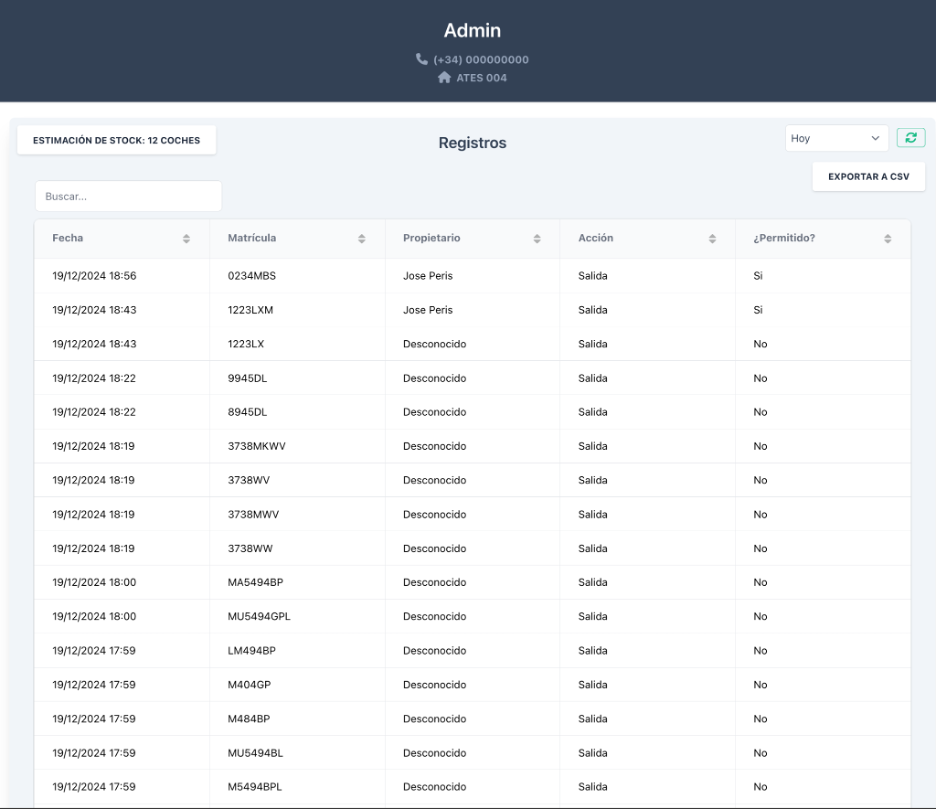
\includegraphics{website_example.png}
		\caption{Website Example.}\label{fig:website_example}
	\end{subfigure}
	\hfill
	\begin{subfigure}{0.45\textwidth}
		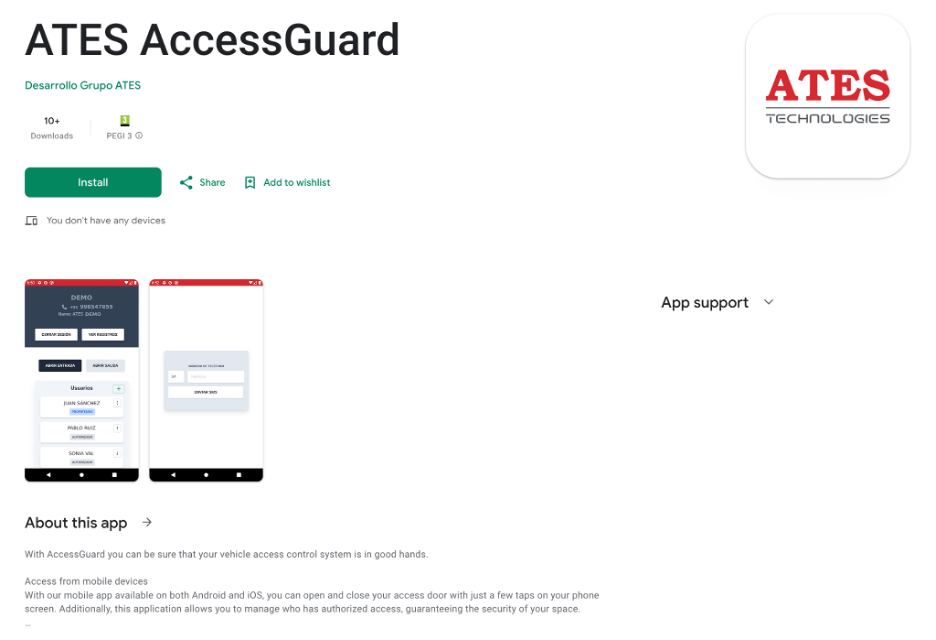
\includegraphics{mobile_app.png}
		\caption{Android Applciation deployed in Google Play Store}\label{fig:mobile_app}
	\end{subfigure}
	\hfill

	\caption{Website design and mobile application.}
\end{figure}

\subsection{Networking}\label{sec:networking}

The interconnection of diverse communities with the web server in a decentralized and user-friendly manner is achieved through the implementation of ZeroTier \autocite{zerotier2025}. This innovative Wide LAN technology facilitates the connection of various devices across the internet by establishing secure VPN tunnels. ZeroTier proves to be an excellent solution for linking different communities to the web server, enabling a range of functionalities such as door access control and license plate recognition.

One of the primary motivations for utilizing EC2 instances in the cloud deployment was the seamless integration of ZeroTier. This approach eliminates the need for proxies or other intermediary measures, streamlining the overall system architecture. The direct installation of ZeroTier alongside the server on EC2 instances ensures a robust and efficient networking solution.

Furthermore, ZeroTier offers the invaluable capability of remote control access. This feature significantly enhances the ability to debug and troubleshoot issues within different communities without the necessity of on-site presence. Technicians and administrators can remotely access the system, diagnose problems, and implement solutions, greatly reducing response times and improving overall system maintenance.

The decentralized nature of ZeroTier aligns well with the project's goals of creating a flexible and scalable network infrastructure. As new communities are added to the system, they can be easily integrated into the existing network topology without major reconfiguration. This scalability ensures that the system can grow organically as more communities adopt the technology.

Security is another crucial aspect addressed by the ZeroTier implementation. The VPN tunnels created by ZeroTier provide encrypted communication channels, safeguarding sensitive data transmitted between the communities and the central web server. This encryption is particularly important when dealing with access control systems and personal information associated with license plate recognition.

In summary, the adoption of ZeroTier as the networking solution for this project offers a powerful combination of ease of use, scalability, remote management capabilities, and enhanced security. These features collectively contribute to a robust and efficient system that can reliably serve multiple communities while remaining adaptable to future growth and technological advancements.


\subsection{User Authentication}\label{sec:authentication}

The authentication system for this project implements a phone-based SMS verification approach, prioritizing both security and user experience. This decision was driven by the requirement to create a simple yet secure authentication process that would be easily accessible to all users, regardless of their technical expertise. Traditional password-based systems often lead to security vulnerabilities due to weak password choices or password reuse, making SMS-based authentication an attractive alternative.

Firebase Authentication was selected as the authentication provider for this implementation, offering a robust and scalable solution for handling SMS-based user verification. This service manages the entire SMS delivery and verification process, including phone number validation, SMS dispatch, and code verification. Firebase's global infrastructure ensures reliable message delivery across different cellular networks and geographical regions, which is crucial for a system deployed across multiple communities.

The authentication flow begins when a user attempts to access the system. They are prompted to enter their phone number, which is then validated for format correctness. Firebase Authentication sends a one-time verification code via SMS to the provided number. This temporary code must be entered by the user within a specified timeframe to complete the authentication process. Upon successful verification, Firebase generates a JSON Web Token (JWT) that serves as the user's authentication credential for subsequent interactions with the system, see \cref{fig:firebase} for reference.

These JWT tokens play a crucial role in maintaining security across the distributed architecture. When a user makes requests to either the cloud server or the terminal servers in specific communities, the JWT token is included in the request headers. The receiving systems verify the token's authenticity using Firebase's public keys, ensuring that only requests from properly authenticated users are processed. The tokens contain encoded information about the user's permissions and access levels, allowing the system to enforce appropriate access controls without requiring additional database queries.

To enhance security further, the tokens are configured with appropriate expiration times, requiring periodic re-authentication. This helps mitigate the risk of token theft or unauthorized access. Additionally, the system maintains a blacklist of revoked tokens to handle cases where immediate access termination is required, such as when a user's privileges are revoked or suspicious activity is detected.

The entire authentication process is integrated seamlessly into both the web interface and mobile applications, providing a consistent user experience across all platforms. Error handling mechanisms are implemented to manage various edge cases, such as failed SMS delivery, network connectivity issues, or invalid verification codes, ensuring that users receive clear feedback and guidance throughout the authentication process.

\begin{figure}
	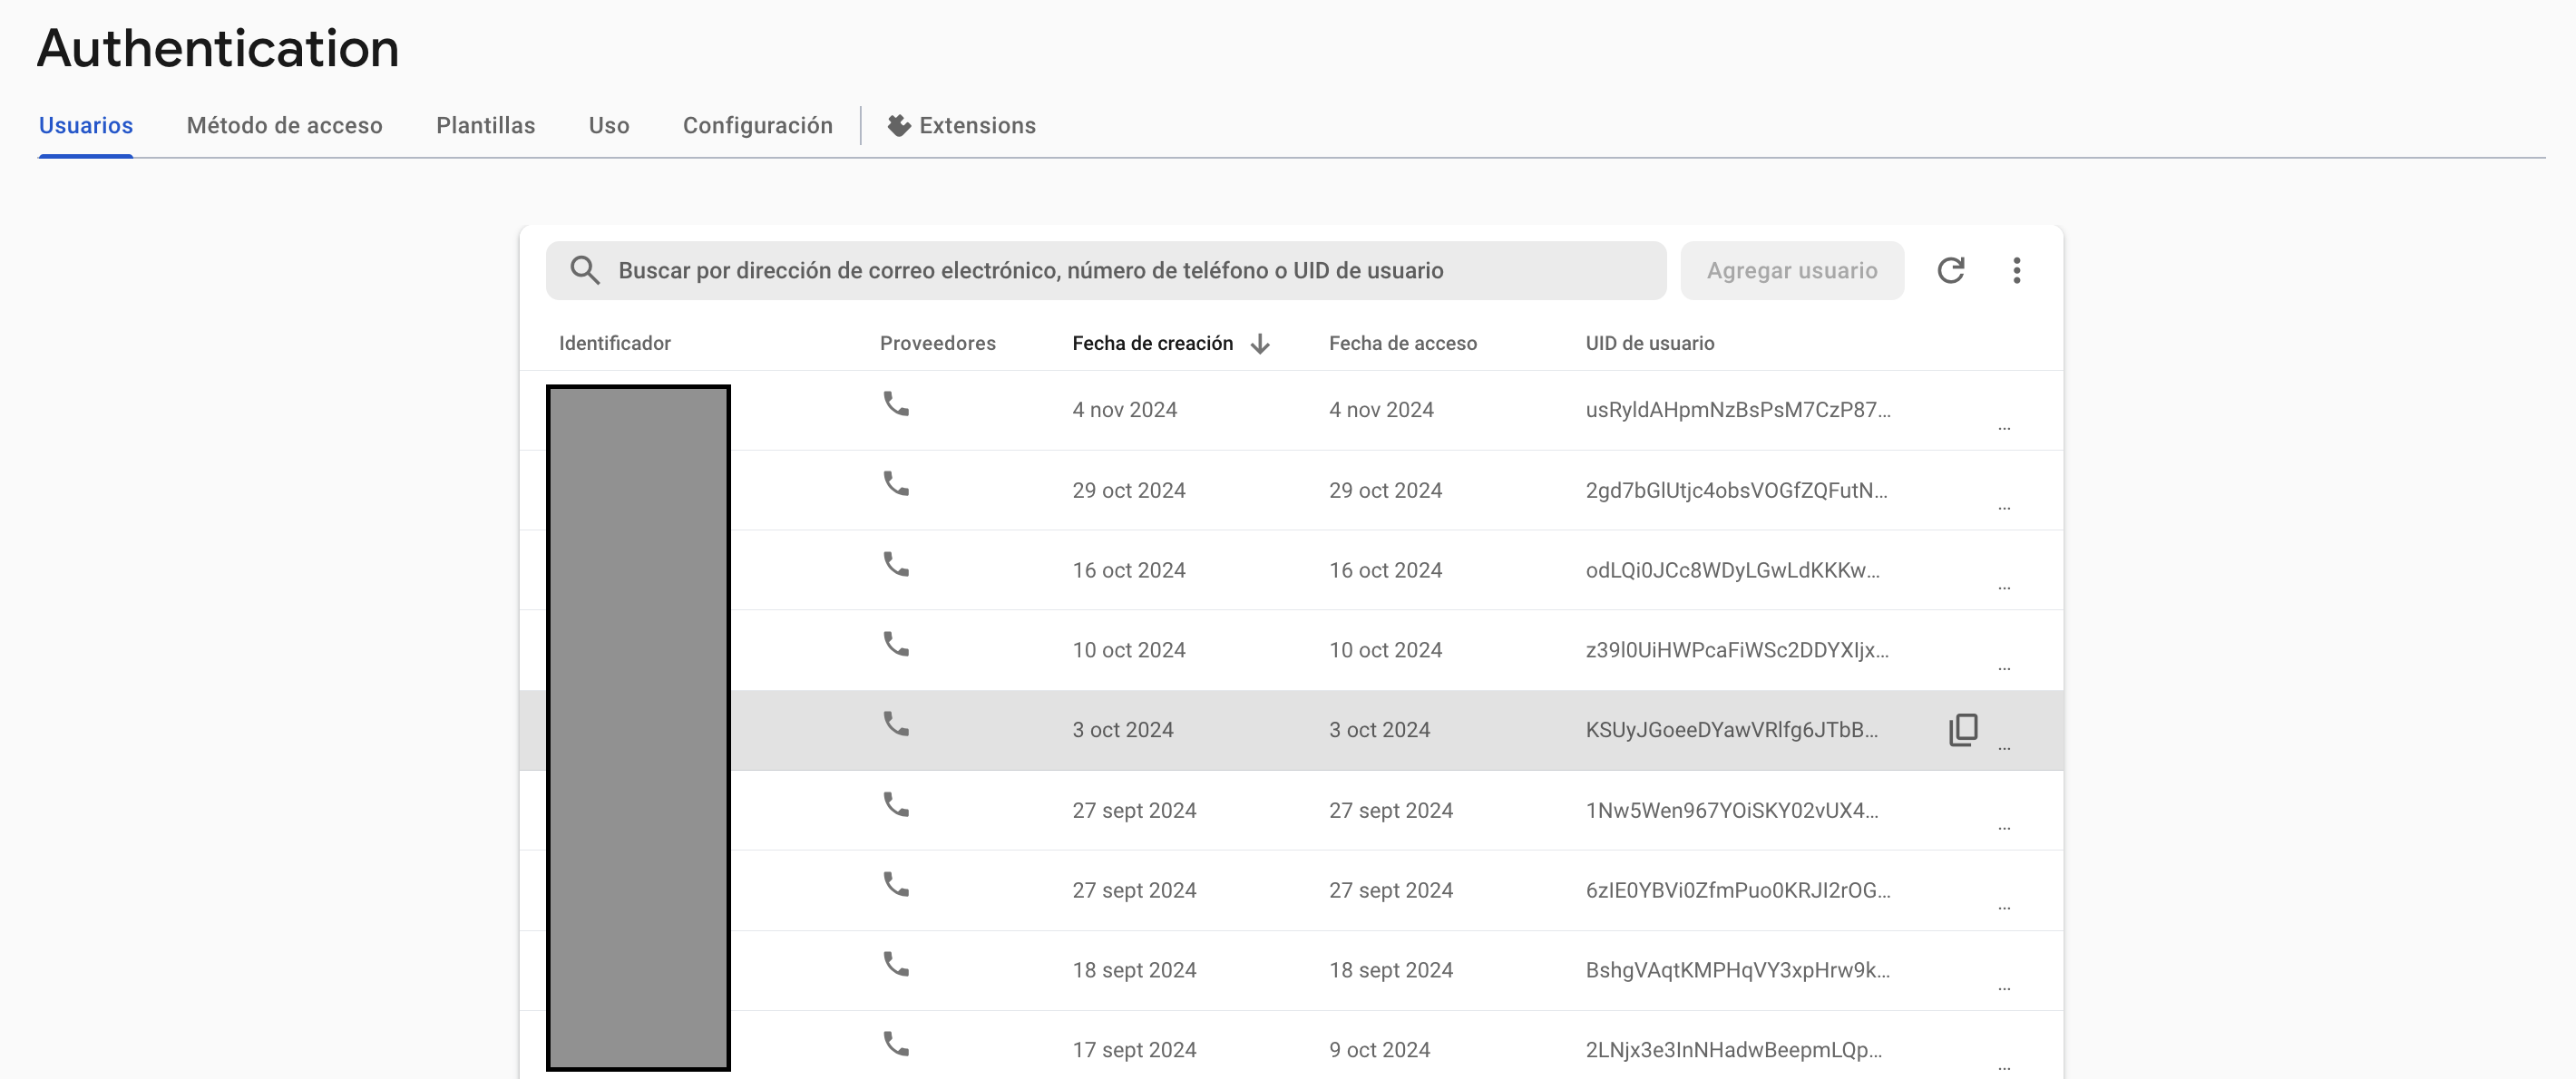
\includegraphics{firebase.png}
	\caption{Firebase Authentication Users example}\label{fig:firebase}
\end{figure}

\section{Deployment}

The deployment process for this distributed parking management system encompasses multiple components, including terminal servers in communities and cloud-based web servers. A standardized approach leveraging modern continuous integration and deployment practices ensures consistent and reliable software updates across all system components. The foundation of this deployment strategy relies on JavaScript frameworks, with applications built and managed through the NPM package manager. To automate the build and release process, a sophisticated GitHub Action pipeline triggers whenever a new release is created in the Git repository. An example can be seen in \cref{fig:github_actions} where web server can be built for the \texttt{0.3.2} version.

\begin{figure}
	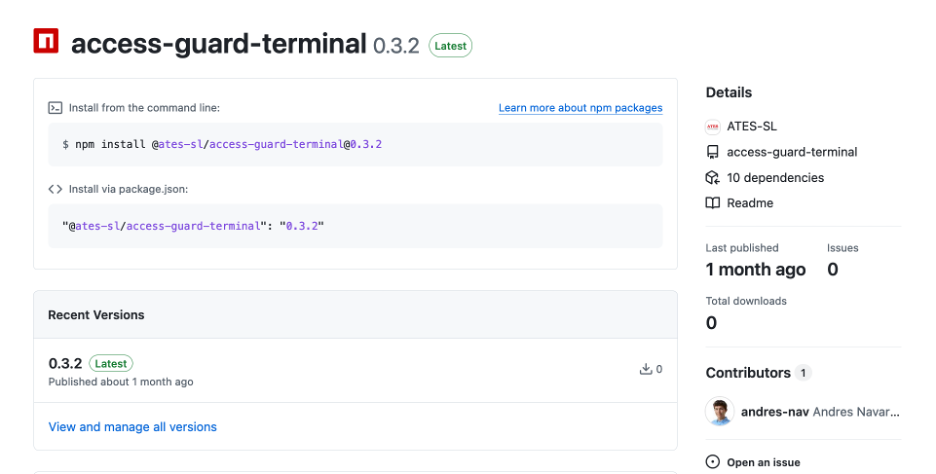
\includegraphics[width=0.7\textwidth]{github_actions.png}
	\caption{Example of the GitHub Actions Pipeline}\label{fig:github_actions}
\end{figure}

The deployment pipeline is designed to handle the complexities of distributing software across various environments while maintaining system integrity and security. When a new version is tagged in the Git repository, the GitHub Actions workflow automatically initiates the build process, creating NPM packages with all necessary dependencies. These packages are then stored in GitHub Packages, providing a centralized and secure location for distribution to both community terminals and cloud servers.

\subsection{Terminal Deployment}

For community terminals, the deployment process requires special consideration due to their distributed nature and the critical importance of maintaining data integrity. The terminal software updates are managed through automated processes, but database migrations present unique challenges. Currently, database migrations are handled manually to ensure data integrity and prevent potential issues that could arise from automated migration processes. This conservative approach reflects the critical nature of the parking management data and the need to maintain system reliability.

While this manual database migration process is functional, it represents an area identified for future improvement. The development team is actively working on designing a robust automated migration system that can maintain data integrity while reducing the operational overhead of manual interventions. This enhancement will need to carefully balance automation with data safety, ensuring that no critical information is lost or corrupted during updates.

\subsection{Server Deployment}

The cloud infrastructure deployment leverages Infrastructure as Code principles through Terraform, enabling consistent and repeatable cloud resource provisioning. This approach allows the entire AWS infrastructure to be defined and managed through version-controlled code, significantly reducing the potential for configuration errors and ensuring deployment consistency across different environments.

A key component of the server deployment strategy is the use of a Baked Amazon Machine Image (AMI) for EC2 instances within the auto-scaling group. This AMI contains all necessary dependencies and application code pre-installed, enabling rapid and reliable instance deployment. When new instances are launched, either during scaling events or updates, they begin with a consistent, production-ready configuration. This approach significantly reduces instance startup time and ensures uniformity across all deployed servers.

\section{Other Considerations}

The implementation of this parking management system necessitates careful consideration of legal and regulatory requirements, particularly those outlined in \cref{ch:regulatory_framework}. To ensure compliance with these regulations, especially the \gls{gdpr}, a comprehensive terms of service and privacy policy framework has been implemented.

The system requires explicit user consent before any personal data collection or processing occurs. This is implemented through a mandatory terms and conditions acceptance process during user registration. The terms of service clearly outline the system's data collection practices, user rights, and privacy protections, ensuring transparency in how personal information is handled. These terms are presented in clear, accessible language to ensure users can make informed decisions about their data.

Data minimization principles are strictly enforced throughout the system's operation. Only essential information required for the parking management functionality is collected and stored. This includes license plate numbers, basic user identification details, and access logs. The system maintains detailed records of user consent and data processing activities, as required by GDPR Article 30, which can be audited to demonstrate compliance with regulatory requirements.

To address the requirements of the ePrivacy Directive and the emerging AI Act, the system implements strict protocols for data retention and processing. All collected data is stored securely with encryption at rest and in transit. The retention period for personal data is clearly defined, and automated processes ensure that data is deleted when it is no longer necessary for the system's operation. This approach aligns with both the data minimization principle and the specific requirements for data retention outlined in the regulatory framework.

Regular updates to the terms of service are conducted to ensure ongoing compliance with evolving regulations and to address new requirements as they emerge. Users are notified of any significant changes to the terms and, where necessary, asked to provide renewed consent. This dynamic approach to legal compliance ensures that the system remains current with regulatory requirements while maintaining transparency with its users.


